\documentclass[12pt]{article}
%\usepackage[T2A,T1,T2A]{fontenc}
\usepackage[utf8]{inputenc}
\usepackage{geometry}
\geometry{verbose,tmargin=3cm,bmargin=3cm,lmargin=3.5cm,rmargin=3.5cm}
\usepackage{float}
\usepackage{amsmath}
\usepackage{amssymb}
\usepackage{graphicx}




\usepackage{multicol}

\usepackage{subfig}

\usepackage[russian]{babel}

\begin{document}

\title{Восстановление параметров с периодическим начальным приближением}
\maketitle

\section{Процесс восстановления параметров модели Курамото}

Напомним процесс восстановления параметров, который мы используем.

Для начала напомним некоторые базовые вещи: общую частоту маятников $ \Omega $ положим $\Omega = 2\pi$ (тогда их период есть $ T =\frac {2\pi} \Omega = 1$). Симметричную разность их частот будем в рамках данной работы считать постоянной и обозначим $ \Delta w$. 

Общее время наблюдения $L=nT$, где $n \in \mathbb{N}$ --- число периодов наблюдения.

Динамика фазовой разницы $ \theta(t)$ описывается следующим дифференциальным уравнением:
\begin{equation}
\dot{\theta}=2\Delta w - k(t)\sin\theta \label{eq:diff}
\end{equation}
с некоторым начальным условием $\theta(0)=init$. Значение начального условия обсудим позднее.

Параметр-функция $k(t)$ (<<каплинг>>) и является центром нашего исследования; ее мы и будем восстанавливать. 

Для этого введем некоторое начальное приближение $k_0(t)$ (опять же, его вид и выбор мы обсудим чуть ниже); решая уравнение \eqref{eq:diff} для $k(t)=k_0(t)$ получим некую функцию $\theta_0(t)$. Заведем два виртульаных маятника:
\[
\begin{cases}
x_{0}(t)=\sin(\Omega t)\\
y_{0}(t)=\sin(\Omega t+\theta_0(t))
\end{cases},
\]
для которых пересчитаем скользящую корреляцию $C_0(t)$ по следующей формуле:
\[
C_{0}(t)=\frac{\int_{t-T/2}^{t+T/2}\sin(\Omega\tau)\sin(\Omega\tau+\theta_{0}(\tau))d\tau}{\sqrt{\int_{t-T/2}^{t+T/2}\sin^{2}(\Omega\tau)d\tau\cdot\int_{t-T/2}^{t+T/2}\sin^{2}(\Omega\tau+\theta_{0}(\tau))d\tau}}
\]
Теперь воспользуемся \textit{гипотезой о квазистационарности}: если \( \theta_0(t) \approx const \), то $C_0 \approx const = \cos \theta_0 $. Поэтому заведем новую переменную:
\[
\phi_0(t)=\arccos C_0(t)
\]
Таким образом одним из замеров качества восстановления можно считать пару \( \theta_0 \) и \(\phi_0 \). Саму же восстановленную параметр-функцию \( \hat{k}(t) \) можно найти из расчета $ \dot{\phi} \approx 0$ (из квазистационарности), откуда
\[
\hat{k}(t)=\frac{2\Delta w}{\sin \phi_0(t)}
\]
Корректность процесса восстановления обеспечивается выполнением основного Курамото-неравенства:
\begin{equation}
\left|\frac{2\Delta w}{k_{0}(t)}\right|\le 1\label{eq:main}
\end{equation}
Теперь разрешим первый из оставшихся вопросов: начальное условие выберем таким, чтобы изначально процедура восстановления была верной, т.е.
\[
init=\arcsin\frac{2\Delta w}{k_0(0)}
\]

\section{Начальное приближение параметр-функции}

Теперь обратимся ко второму оставленному вопросу: а именно к выбору $k_0(t)$.

Было предложено исследовать семейство начальных приближений вида:
\[
k_0(t)=A \cos(Bt+\delta) + C
\]
где $A$ --- амплитуда, $B$ его частота, $C$ вертикальный сдвиг. Переменная $\delta$ здесь служит для сдвига начальной фазы параметр-функции относительно фазы основных маятников. Отсюда можно получить несколько разовых ограничени:
\begin{itemize}
	\item $k_0(t) \ge 0$, а значит $-A+C \ge 0$;
	\item основное Курамото неравенство выполняется, если 
	\[
	2\Delta w \le A\cos (Bt+\delta)+C \Rightarrow 2 \Delta w \le A+C;
	\]
	\item в начальный момент времени основное Курамото-неравенство не должно нарушаться:
	\[
	2 \Delta w \le A\cos \delta + C;
	\]
	\item предполагается, что качественное восстановление возможно только лишь при $B\ll \Omega$. Для удобства далее мы везде будем мерить $B$ в долях $\Omega$.
\end{itemize}

Приведем вид графиков при разных параметрах (попадание $k_0(t)$ ниже красной линии $2\Delta w$ означает нарушение основного неравенства):
\begin{figure}[H]
	\centering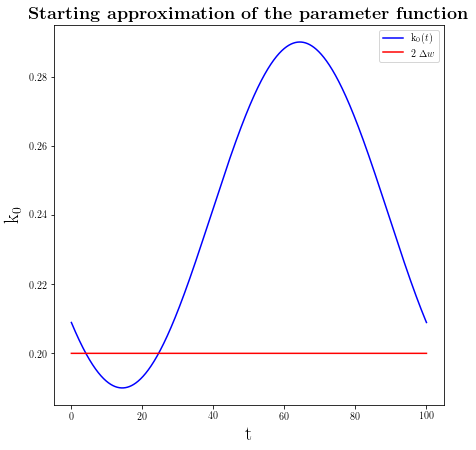
\includegraphics[width=0.6\columnwidth]{im1.png}\caption{Начальное приближение $k_0(t)$ при $n=100$, $\Delta w=0.1$, $A=0.05$, $B=\frac{1}{100}\Omega$, $\delta = \pi - 0.9$, $C=0.24$ }
\end{figure}
\begin{figure}[H]
	\centering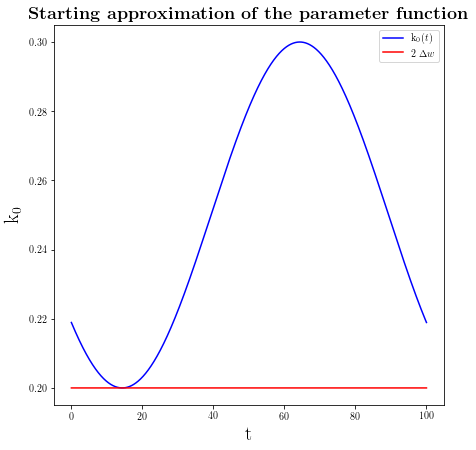
\includegraphics[width=0.6\columnwidth]{im2.png}\caption{Начальное приближение $k_0(t)$ (случай касания) при $n=100$, $\Delta w=0.1$, $A=0.05$, $B=\frac{1}{100}\Omega$, $\delta = \pi - 0.9$, $C=0.25$ }
\end{figure}
\begin{figure}[H]
	\centering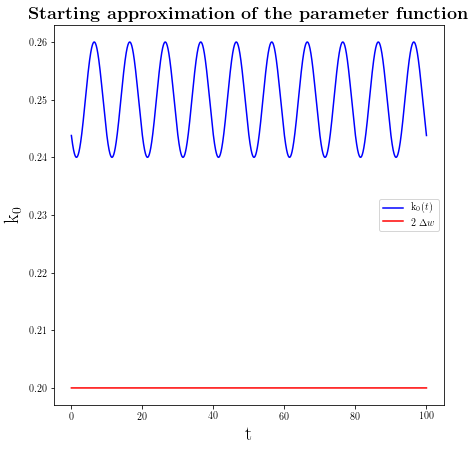
\includegraphics[width=0.6\columnwidth]{im3.png}\caption{Начальное приближение $k_0(t)$ (случай полного попадания) при $n=100$, $\Delta w=0.1$, $A=0.01$, $B=\frac{1}{10}\Omega$, $\delta = \pi - 0.9$, $C=0.25$ }
\end{figure}

\paragraph{Качество.} Теперь прежде чем заговорить о результатах восстановления, введем относительное качество восстановления для $\mathbb{L}_2$ метрики:
\[
q=\frac{\int_0^L (\hat{k}-k_0)^2 dt}{\int_0^L (k_0-\overline{k_0})^2 dt}
\]

\section{Примеры восстановления}
Прежде чем начать немного поясним: для каждого набора входных данных приводится три картинки, параметр-функция, для $\phi_0$ и $\theta_0$ и для $\hat{k}(t)$ и $k_0(t)$; для последней пары посчитан $q$.

Из всего дальнейшего следует три основных вывода:
\begin{itemize}
	\item восстановление по фазовой разности выглядит довольно корректно;
	\item восстановление итогового параметра $\hat{k}$, видимо, требует иного пересчет из $\phi_0$;
	\item вероятно, стоит пересмотреть метод подсчета качества (хотя она может быть и удовлетворительной при исправленном методе восстановления).
\end{itemize}
\begin{figure}[H]
	\centering
	\begin{centering}
		\subfloat[$k_0(t)$]{\centering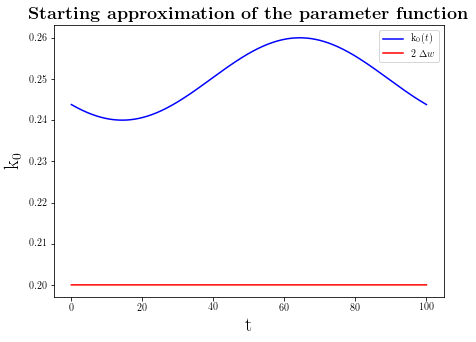
\includegraphics[width=0.6\columnwidth]{im6.png}}
	\end{centering}
	\begin{centering}
		\subfloat[$\phi_0$ и $\theta_0$]{\centering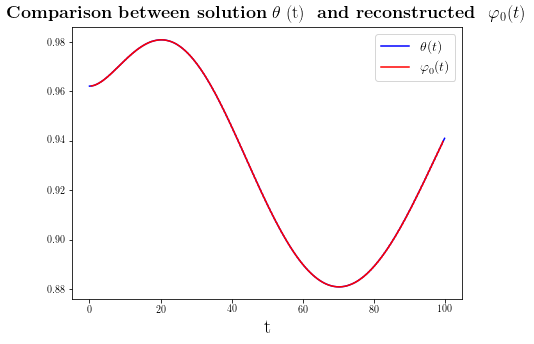
\includegraphics[width=0.6\columnwidth]{im4.png}}
	\end{centering}
	\begin{centering}
		\subfloat[$\hat{k}(t)$ и $k_0(t)$]{\centering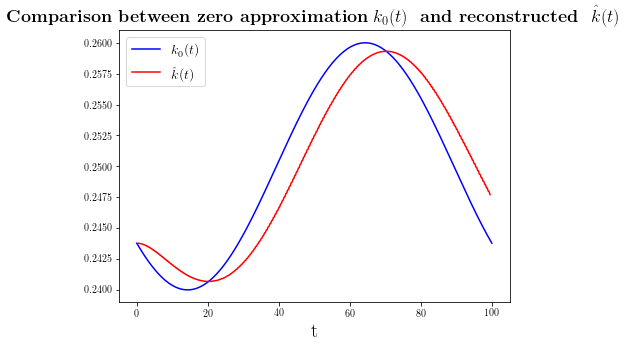
\includegraphics[width=0.7\columnwidth]{im5.png}}
	\end{centering}
	\caption{Процесс восстановления для $n=100$, $\Delta w=0.1$, $A=0.01$, $B=\frac{1}{100}\Omega$, $\delta = \pi - 0.9$, $C=0.25$. Результат: $q=0.13$}
\end{figure}

\begin{figure}[H]
	\centering
	\begin{centering}
		\subfloat[$k_0(t)$]{\centering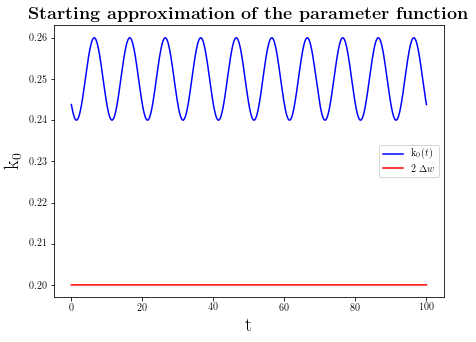
\includegraphics[width=0.6\columnwidth]{im7.png}}
	\end{centering}
	\begin{centering}
		\subfloat[$\phi_0$ и $\theta_0$]{\centering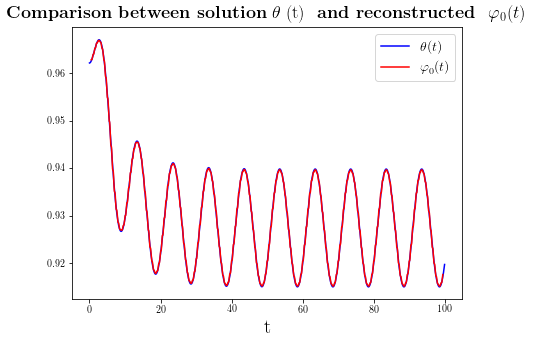
\includegraphics[width=0.6\columnwidth]{im8.png}}
	\end{centering}
	\begin{centering}
		\subfloat[$\hat{k}(t)$ и $k_0(t)$]{\centering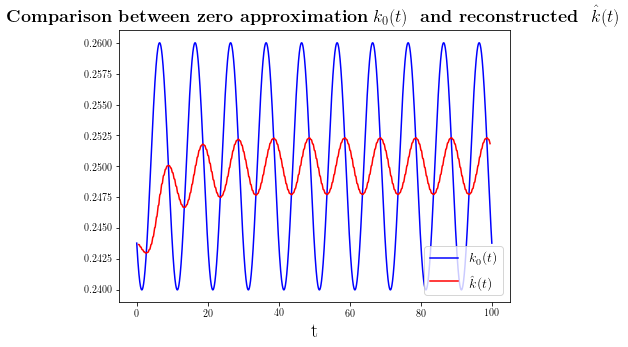
\includegraphics[width=0.7\columnwidth]{im9.png}}
	\end{centering}
	\caption{Процесс восстановления для $n=100$, $\Delta w=0.1$, $A=0.01$, $B=\frac{1}{10}\Omega$, $\delta = \pi - 0.9$, $C=0.25$. Результат: $q=0.95$}
\end{figure}

\begin{figure}[H]
	\centering
	\begin{centering}
		\subfloat[$k_0(t)$]{\centering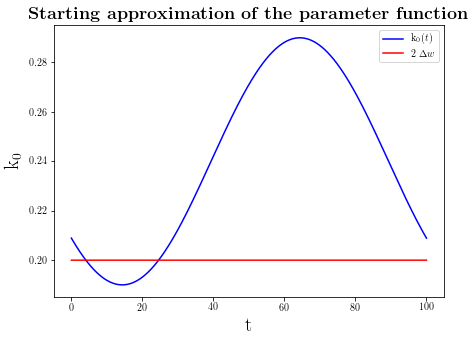
\includegraphics[width=0.6\columnwidth]{im10.png}}
	\end{centering}
	\begin{centering}
		\subfloat[$\phi_0$ и $\theta_0$]{\centering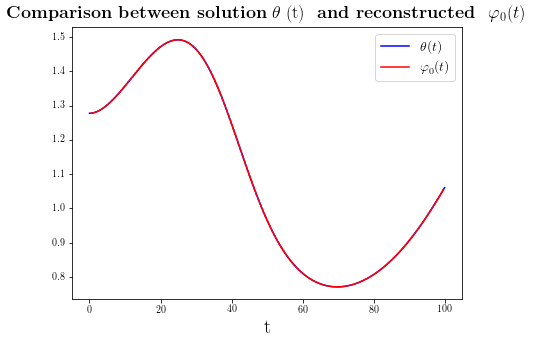
\includegraphics[width=0.6\columnwidth]{im11.png}}
	\end{centering}
	\begin{centering}
		\subfloat[$\hat{k}(t)$ и $k_0(t)$]{\centering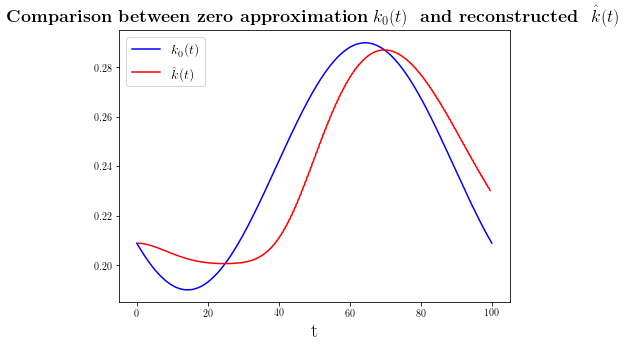
\includegraphics[width=0.7\columnwidth]{im12.png}}
	\end{centering}
	\caption{Процесс восстановления для $n=100$, $\Delta w=0.1$, $A=0.05$, $B=\frac{1}{100}\Omega$, $\delta = \pi - 0.9$, $C=0.24$. Результат: $q=0.225$}
\end{figure}

\begin{figure}[H]
	\centering
	\begin{centering}
		\subfloat[$k_0(t)$]{\centering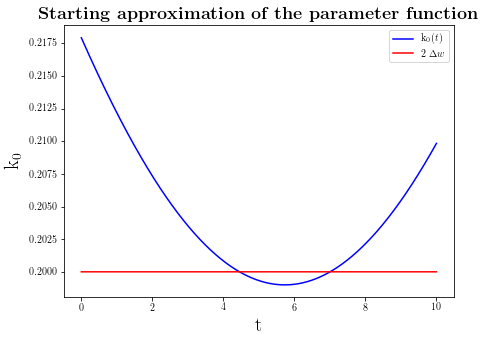
\includegraphics[width=0.6\columnwidth]{im13.png}}
	\end{centering}
	\begin{centering}
		\subfloat[$\phi_0$ и $\theta_0$]{\centering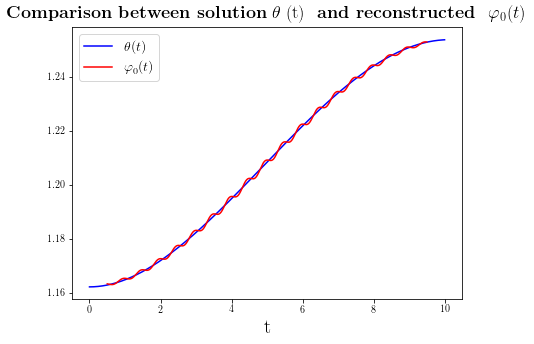
\includegraphics[width=0.6\columnwidth]{im14.png}}
	\end{centering}
	\begin{centering}
		\subfloat[$\hat{k}(t)$ и $k_0(t)$]{\centering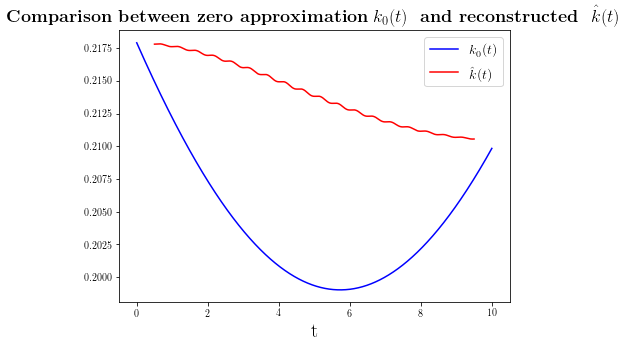
\includegraphics[width=0.7\columnwidth]{im15.png}}
	\end{centering}
	\caption{Процесс восстановления для $n=10$, $\Delta w=0.1$, $A=0.05$, $B=\frac{1}{40}\Omega$, $\delta = \pi - 0.9$, $C=0.249$. Результат: $q=7.117$}
\end{figure}

\end{document}
